%(BEGIN_QUESTION)
% Copyright 2006, Tony R. Kuphaldt, released under the Creative Commons Attribution License (v 1.0)
% This means you may do almost anything with this work of mine, so long as you give me proper credit

I denne kontinuerlige kjeksbakeprosessen blir kjeks transportert gjennom en ovn på et transportbånd. Temperaturen på kjeksen måles etter at den har passert ovnen. Et kontaktløst termometer (infrarødt pyrometer) brukes til målingen, slik at sensoren ikke kommer i kontakt med maten.

$$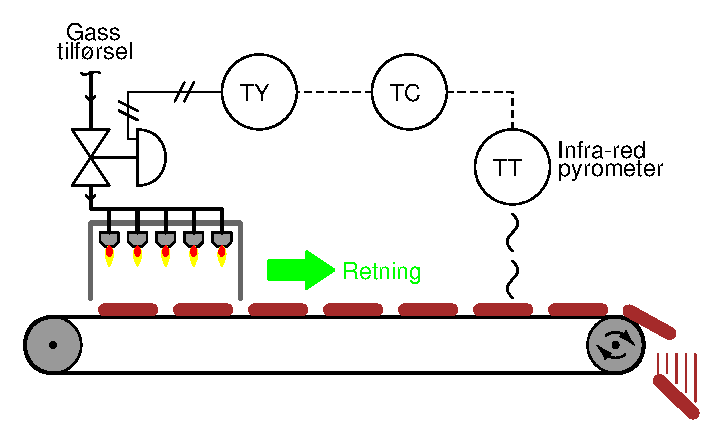
\includegraphics[width=15.5cm]{i00110x01.eps}$$

Anta at transporttiden fra kjeksen forlater ovnen til den når pyrometeret er 15 sekunder. Hva kalles denne tiden i reguleringsteknikk, og hvilken effekt har den på systemets stabilitet?

\vskip 20pt \vbox{\hrule \hbox{\strut \vrule{} {\bf Forslag til sokratisk diskusjon} \vrule} \hrule}

\begin{itemize}
\item{} Forklar hvordan du kan forbedre ytelsen til dette reguleringssystemet.
\item{} Forklar hvordan temperatursenderen (TT) måler kjekstemperaturen. Hvilke fysiske prinsipper bruker senderen i målingen?
\end{itemize}

\underbar{file i00110}
%(END_QUESTION)





%(BEGIN_ANSWER)

Denne forsinkelsen kalles vanligvis {\it dødtid} (eller {\it transportforsinkelse}), og den skaper store problemer for tilbakekoblede reguleringssystemer fordi regulatoren bare ser de forsinkede resultatene av egen reguleringshandling. Dette er analogt med å kjøre bil ved å se {\it bakover} ut bakruten og styre ut fra veien du allerede har kjørt over.

%(END_ANSWER)





%(BEGIN_NOTES)

Problemet i dette systemet er ikke tiden kjeksen er i ovnen, men tiden den bruker mellom ovnsutløpet og punktet der den måles av den infrarøde temperatursenderen. Denne forsinkelsen kalles «dødtid», og det er uheldig i alle reguleringssystemer.

Dødtid bør elimineres fra prosessløkker der det er mulig, på samme måte som dødgang og hysterese bør elimineres i prosessinstrumenter (sendere og ventiler). Slike «døde» effekter får prosessen til å virke helt uresponsiv innenfor et visst tidsrom eller område. Siden et grunnprinsipp i prosesstyring er at du ikke kan regulere det du ikke måler, betyr dette at ovnsreguleringen ikke kan kontrollere faktisk kjekstemperatur i sanntid. Den kan i beste fall regulere temperaturen 15 sekunder senere, som betyr at den kan over- eller underbake kjeks uten å oppdage det før 15 sekunder {\it etter} at skaden er skjedd.

\vskip 10pt

En enkel løsning er å flytte temperatursenderen nærmere ovnsutløpet slik at den «ser» kjeks idet den kommer ut, i stedet for 15 sekunder senere. Det kan imidlertid være at infrarød stråling fra flammene i ovnen «lurer» senderen til å «tro» at kjeksen er varmere enn den faktisk er, noe som vil påvirke reguleringskvaliteten.

En ny løsning foreslått av en student var å bruke {\it to} transportbånd i stedet for ett, der bånd nummer to går mye raskere enn båndet gjennom ovnen. Det vil redusere dødtiden uten å redusere steketiden i ovnen:

$$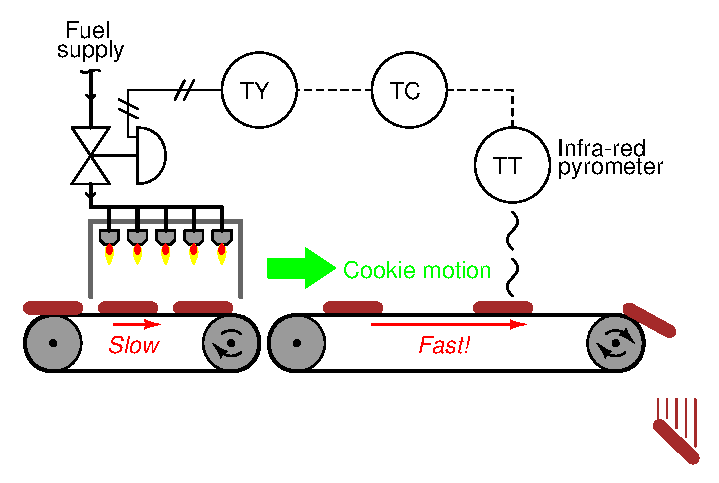
\includegraphics[width=15.5cm]{i00110x02.eps}$$

En annen løsning er å måle temperaturen på transportbåndet inne i ovnen (for eksempel med en infrarød temperatursender plassert på undersiden av båndet, skjermet mot direkte og reflektert stråling fra brennerne). Dette er ikke like godt som direkte måling av kjeks, men har fordelen at man måler en temperatur som kan reguleres umiddelbart, i stedet for en tidsforsinket temperatur.

%INDEX% Control, basics: process dead time
%INDEX% Process: cookie baking oven

%(END_NOTES)
